\documentclass{article}
\usepackage{graphicx} % Required for inserting images
\usepackage{geometry}
\usepackage[T1]{fontenc}
\usepackage[utf8]{inputenc}

\renewcommand{\figurename}{Slika}

\title{Bachelor Thesis}
\author{Ivan Jevtic}
\date{September 2024}

\begin{document}

   % Title Page
   \newgeometry{top=1in, bottom=1in, left=1in, right=1in} % New margins for title page
   \begin{titlepage}
      \begin{center}
         
         % add your university logo here
         % negative value moves the logo up
         \vspace*{-1in}
         \includegraphics[width=0.4\textwidth]{raf_logo.png}

         % set font size to 14pt
         \vspace{1in}
         \Large
         \textbf{DIPLOMSKI RAD}
         
         % set horizontal margin for the title to 1.5in and center it
         \vspace{1in}
         \Huge
         \textbf{Razvoj višekorisničkog kolaborativnog editora}
         
         \vspace{1in}


         \fontsize{14pt}{18pt}\selectfont
         \textbf{Ivan Jevtić} \\
         \textbf{RN 4/2020}
         \vspace*{1.5in}
         
         \begin{center}
            \normalsize
            \begin{tabular}{p{0.7\textwidth} p{0.5\textwidth}}
               \fontsize{14pt}{18pt}\selectfont   
               \textbf{Mentor:} & 
            
               \fontsize{14pt}{18pt}\selectfont
               \textbf{Komisija:} \\
               dr Miloš Radenković & dr Miloš Radenković \\
                                 
            \end{tabular}
         \end{center}

         \vspace*{\fill}

         \normalsize
         Beograd, septembar 2024.


         
      \end{center}
   \end{titlepage}
   \restoregeometry % Restore original margins

   \newpage
   \newgeometry{top=1.3in, bottom=2.2in, left=1.4in, right=1.4in} % New margins for title page
   
   % Table of Contents
   \renewcommand{\contentsname}{Sadržaj}
   \addtocontents{toc}{\protect\thispagestyle{empty}}
   \tableofcontents
   \thispagestyle{empty} % Remove page numbers

   \restoregeometry % Restore original margins

   \newpage
   
    \thispagestyle{empty} % Remove page number from Abstract page
    
    % Define a command to format a specific section title
    \newcommand{\specialsection}[1]{
       \section*{\centering{#1}} % Center and italicize the section title
    }
    
    \vspace*{0.5in}
    \specialsection{Apstrakt}
    
    \vspace*{0.5in}

    Ovaj diplomski rad istražuje \textbf{višekorisničke kolaborativne editore}, sisteme koji omogućavaju istovremenu saradnju više korisnika na istom dokumentu u realnom vremenu. U uvodnom delu rada, pružen je detaljan pregled osnovnih principa ovih sistema, uključujući \textbf{sinhronizaciju promena}, \textbf{upravljanje konfliktima} i \textbf{održavanje doslednosti} između različitih korisnika. Takođe, analizirani su postojeći alati i rešenja, kao što su \textbf{Google Docs} i \textbf{Microsoft Office Online}, zajedno sa njihovim prednostima i manama.
    
    Rad se zatim fokusira na razvoj prilagođenog višekorisničkog kolaborativnog editora. Opisuje se \textbf{arhitektura rešenja}, korišćeni \textbf{algoritmi} za sinhronizaciju podataka, kao i izazovi u vezi sa \textbf{performansama} i \textbf{bezbednošću}. Prikazani su rezultati eksperimenata koji testiraju efikasnost razvijenog sistema, zajedno sa diskusijom o njegovoj primeni u stvarnim uslovima i mogućnostima za dalja unapređenja.

   \newpage

   \newpage
   \pagenumbering{arabic}
   \setcounter{page}{1}

   \section{Uvod}

   \vspace{+0.5cm}
   
   \subsection{Istorija i motivacija}
   

    \subsubsection{Rani razvoj kolaborativnih editora (1970-1980)}

    Ideja kolaborativnih editora, koji omogućavaju više korisnika da istovremeno rade na istom dokumentu, počela je da se razvija tokom 1970-ih godina, u vreme kada su naučnici i inženjeri počeli da istražuju potencijal multi-korisničkih sistema. Ova era bila je obeležena pionirskim radom na sistemima koji su nastojali da olakšaju istovremenu saradnju između korisnika, mada je razvoj tih tehnologija bio ograničen dostupnim resursima, kao što su niska brzina mrežnih veza i ograničena računska snaga.
    
    Jedan od prvih važnih koraka u ovom pravcu bio je razvoj \textbf{NLS sistema (oN-Line System)}, koji je predstavio \textbf{Daglas Engelbart} 1968. godine.

    \paragraph{}
    \textbf{NLS sistem}, poznat kao \textbf{oN-Line System (NLS)}, razvijen je zahvaljujući finansiranju od strane DARPA-e i Ratnog vazduhoplovstva SAD-a. NLS je zamišljen od strane \textbf{Daglasa Engelbarta} i razvijen u saradnji sa njegovim kolegama iz \textbf{Stanford Research Institute} (SRI). Ovaj sistem je prvi uveo koncept \textbf{hipertekstualnih linkova}, \textbf{miša}, \textbf{raster-sken monitora}, organizaciju informacija po relevantnosti, \textbf{prozor na ekranu} (windowing), prezentacione programe i mnoge druge koncepte koji su danas sastavni deo savremenih računarskih sistema.
    
    Dana \textbf{9. decembra 1968.}, Engelbart je javnosti predstavio NLS sistem u San Francisku, na \textbf{Fall Joint Computer Conference}, događaju koji je kasnije postao poznat kao \textit{"Majka svih demonstracija"} zbog brojnih revolucionarnih funkcija koje su tom prilikom prvi put prikazane. Engelbartov terminal bio je povezan sa video projekcijom velikog formata, pozajmljenom od NASA Ames Research Center, a putem telefonskih linija povezan je sa SDS 940 računarom u Menlo Parku, Kalifornija, na udaljenosti od 30 milja, gde se nalazio \textbf{Augmentation Research Center}, koji je Engelbart osnovao u SRI.
    
    Na ekranu visokom skoro \textbf{7 metara}, sa video umecima, publika je mogla da vidi kako Engelbart upravlja mišem, dok su se članovi njegovog tima iz Menlo Parka pridruživali prezentaciji u realnom vremenu. Dolaskom ARPA mreže u SRI 1969. godine, tehnologija vremenskog deljenja resursa (time-sharing) postala je nepraktična za distribuciju među većim brojem korisnika, ali je NLS otvorio put ka razvoju savremenih informacionih tehnologija koje danas koristimo.
    
    \begin{figure}[h]
        \centering
        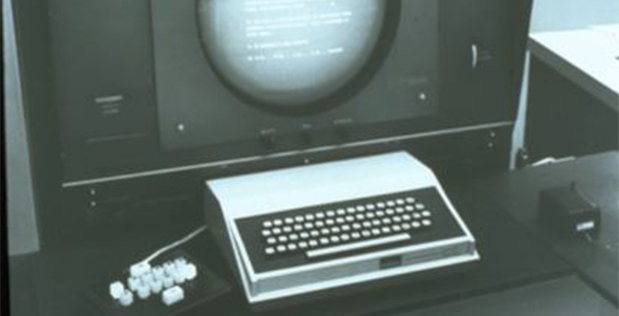
\includegraphics[width=0.8\textwidth]{nls.jpg}
        \caption{Daglas Engelbart tokom "Majke svih demonstracija", 1968.}
        \label{fig:nls_demo}
    \end{figure}

    
    Iako NLS nije bio kolaborativni editor u savremenom smislu, predstavljao je revolucionaran koncept koji je omogućavao zajedničko pregledanje i uređivanje dokumenata. Ovaj sistem je pokazao kako bi računar mogao postati alat za grupni rad, posebno u organizacijama sa složenim informacionim potrebama. Engelbartova vizija o umreženoj saradnji postavila je temelj za dalji razvoj kolaborativnih editora, ali su tehnološka ograničenja tog vremena sprečila njegovu široku primenu.
    
    U toku 1970-ih i ranih 1980-ih, nekoliko naučnih radova i istraživanja pokušalo je da reši problem zajedničkog uređivanja dokumenata. Međutim, zbog ograničenih mrežnih kapaciteta i činjenice da internet još uvek nije bio široko dostupan, razvoj je bio fokusiran na lokalne mreže i eksperimentalne sisteme. Primer toga bio je konceptualni okvir poznat kao \textbf{"Shared Workspace"}, koji je omogućavao korisnicima da dele radno okruženje i informacije u realnom vremenu. Ovi rani sistemi su omogućavali deljenje sadržaja, ali nisu nudili dinamičko uređivanje, koje je karakteristično za modernu kolaboraciju.

    \paragraph{}
    Tokom kasnih 1980-ih, tehnologija je značajno napredovala, a računarstvo je postajalo sve moćnije i pristupačnije. Ova era je videla pojavu prvih pravih kolaborativnih editora. Jedan od prvih sistema koji je omogućio više korisnika da uređuju dokumente u realnom vremenu bio je \textbf{GROVE (Group Outline Viewing Editor)}, razvijen 1989. godine. GROVE je omogućavao simultano uređivanje strukturisanih dokumenata i predstavljao je jedan od pionirskih sistema za kolaborativno uređivanje. Iako je bio ograničen na lokalne mreže, zbog nedostatka interneta i infrastrukture za širu mrežnu primenu, GROVE je pokazao kako bi kolaboracija mogla funkcionisati u okruženju sa više korisnika.

    GROVE omogućava prikazivanje više pogleda na konturu, gde se svaki prikaz prikazuje u grupnom prozoru koji može biti repliciran na više mašina. Ovi prikazi mogu biti privatni, deljeni ili javni, u zavisnosti od potreba korisnika. Značajna karakteristika GROVE sistema je njegov grupni prozor, koji prikazuje prisustvo i aktivnost svih učesnika koji rade na dokumentu. U ovom zajedničkom prostoru korisnici mogu izvršavati standardne operacije uređivanja, kao što su umetanje, brisanje, sečenje i lepljenje teksta. Sistem takođe nudi napredne funkcionalnosti, poput proširivanja i skupljanja delova konture, kao i promene dozvola za čitanje i pisanje specifičnih stavki.

    \begin{figure}[h]
        \centering
        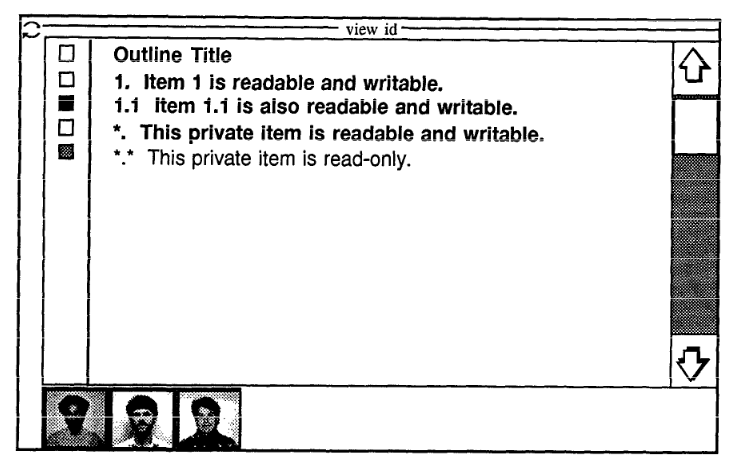
\includegraphics[width=0.8\textwidth]{grove.png}
        \caption{Grove grupni prozor, 1989.}
        \label{fig:nls_demo}
    \end{figure}

    Jedna od ključnih karakteristika GROVE sistema je kolaboracija u realnom vremenu—svaka promena koju napravi jedan učesnik odmah je vidljiva ostalima, osiguravajući da svi učesnici budu u toku sa najnovijim izmenama. Ovaj mehanizam povratne informacije u realnom vremenu bio je od suštinskog značaja za kreiranje visoko interaktivnog i responzivnog okruženja.
    
    Za razliku od sistema u realnom vremenu kao što je GROVE, drugi sistemi tog vremena, poput CES-a, Quilta ili Shared Books-a, omogućavali su kolaborativno uređivanje dokumenata, ali su radili u asinhronom režimu. Ovi sistemi su dozvoljavali korisnicima da rade na različitim delovima dokumenta, često tokom dužih perioda, što je omogućavalo manje fokusirane sesije. Distinkcija između kolaborativnih sistema u realnom i asinhronom vremenu postala je važan fokus u proučavanju kolaborativnih sistema.
    
    GROVE-ova mogućnost uređivanja u realnom vremenu, uz podršku za upravljanje različitim prikazima i korisničkim dozvolama, učinila ga je značajnim korakom u razvoju sistema za grupni rad.
    
    Pored GROVE-a, nekoliko drugih projekata je nastalo u ovom periodu, ali su svi imali slične izazove – mrežna infrastruktura nije bila dovoljno razvijena za globalnu kolaboraciju, a računarstvo nije bilo dovoljno moćno da podrži složene algoritme potrebne za rešavanje problema sinkronizacije i konzistentnosti podataka među korisnicima.
    
    Dakle, tokom 1970-ih i 1980-ih godina, iako su načinjeni značajni koraci u pravcu kolaborativnih sistema, ovi rani pokušaji su uglavnom ostali ograničeni na istraživačke laboratorije i specifične upotrebe unutar lokalnih mreža. Tek kasnije, sa razvojem interneta i većom dostupnošću mrežnih resursa, kolaborativni editori su počeli da ostvaruju svoj puni potencijal.
    
   

\end{document}
